\chapter{CMOS VLSIにおける電力とSOTB技術}
{
\label{chap:vlsi}
\section{消費電力}
\label{sec:power}
半導体技術の向上により集積度の高い集積化路が広く用いられるようになった。集積度の高い集積化路をVLSI(Very Large Scale Integration)と呼ぶ。VLSIでは何十万以上ものトランジスタが1チップ上に搭載されている。集積度を向上させることにより高い性能を実現する一方で、その主な問題は消費電力の増加であった。そのような背景から現在ではnMOSトランジスタとpMOSトランジスタを相補的に組み合わせて構成するCMOSプロセスが広く使われている。一般にCMOSを用いたVLSIの電力消費は2つの要素に分けることができる。
\begin{itemize}
\item ダイナミック消費電力$P_{dynamic}$
\item スタティック消費電力$P_{static}$
\end{itemize}

つまり、全体の消費電力$P_{total}$との関係は
\begin{eqnarray}
P_{total} = P_{dynamic} + P_{static}
\end{eqnarray}
である。
\subsection{ダイナミック電力}
\label{subsec:dynamic_power}
ダイナミック電力の要因は以下の2種類に分類できる。
\begin{itemize}
\item ゲートのスイッチングにより発生する負荷容量への充放電
\item pMOSとnMOSが同時にオンとなることにより発生する貫通電流
\end{itemize}
ただし大部分のダイナミック電力は前者のスイッチング電力である。このスイッチング電力を$P_{switching}$とすると以下の式で表される。\cite{west}
\begin{eqnarray}
P_{switching} = \alpha C V^2_{DD}f
\end{eqnarray}
ここで$\alpha$は活性化率と呼ばれ回路中で0から1へ遷移する確率、$C$は負荷容量、$V_{DD}$は電源電圧である。

\subsection{グリッチ}
\label{subsec:glitch}
直列に回路を接続する構造の場合、グリッチと呼ばれる信号変化により発生する電力を考慮する必要がある。グリッチによる信号変化は本来不要なものであるがビット間の遅延時間の差により発生してしまう。図\ref{fig:glitch}はCMAのPEにおいて積算を行った時の波形である。左の赤い線が演算が開始した時刻であり、右の赤い線が演算の完了時刻を表している。最終的な値に確定するまでの間に不要なスイッチングが発生しているのが確認できる。組み合わせ回路の規模が大きくなり、複雑化すれほどグリッチの影響は大きくなる。このグリッチによる消費電力は全体の消費電力の40\%以上を占めることもあり、グリッチを取り除くことが消費電力削減に有効である。\cite{glitch}

\begin{figure}[h]
\centering
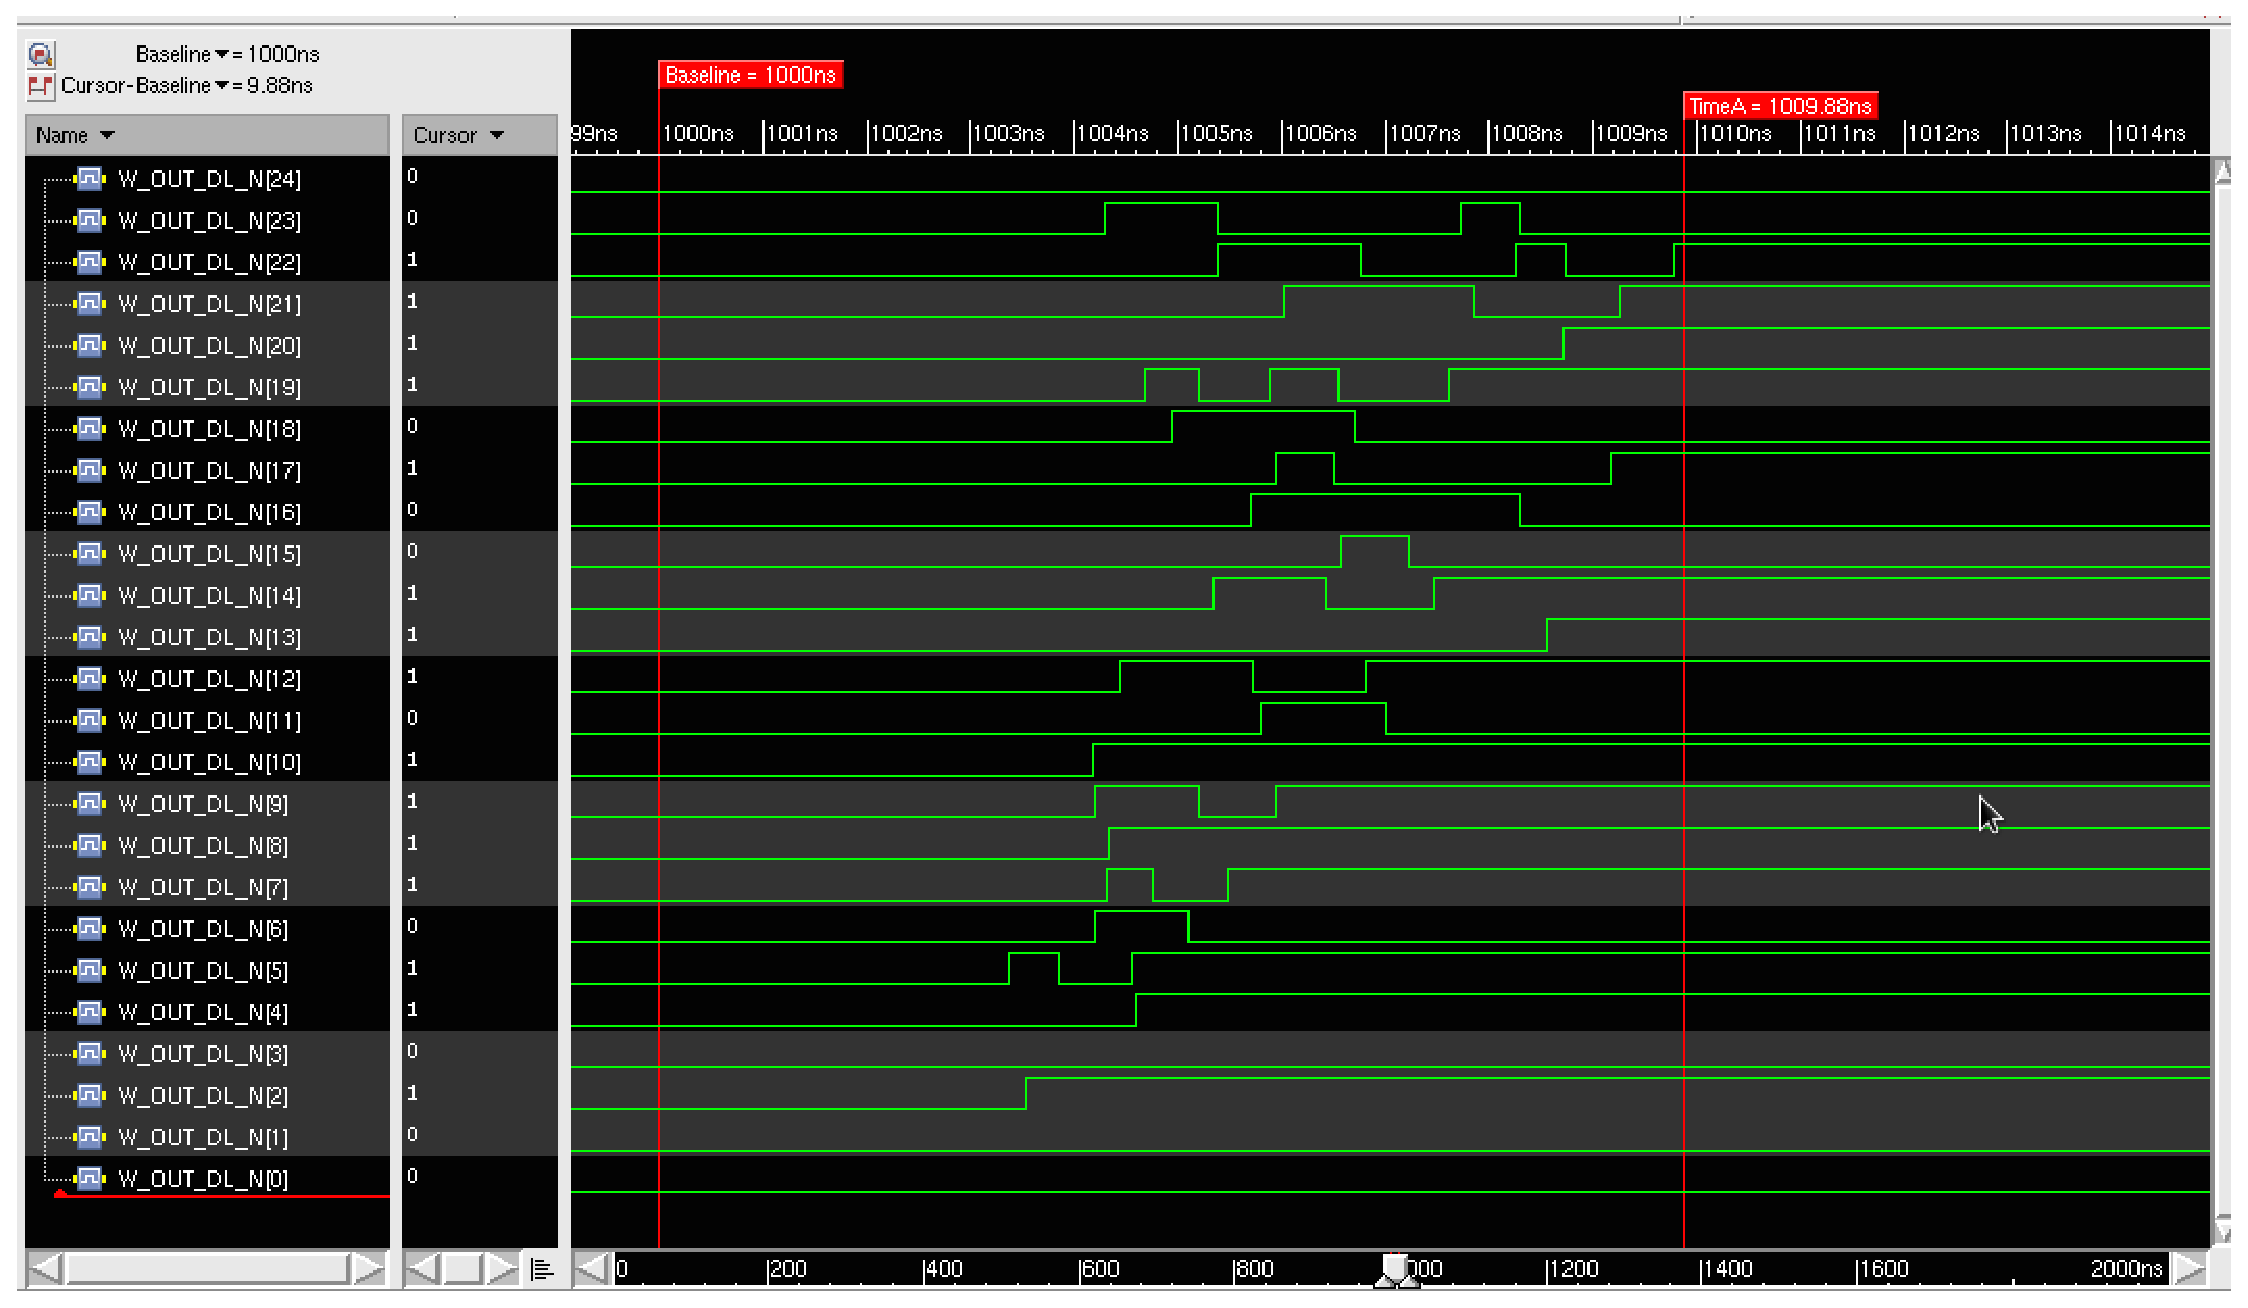
\includegraphics[width=12cm]{./chap2/fig/glitch.eps}
\caption{グリッチの様子}
\label{fig:glitch}
\end{figure}

\subsection{スタティック電力}
\label{subsec:static_power}
スタティック電力はスイッチングしていないときにも消費される電力である。スイッチングしていないときに流れる電流をリーク電流と呼び。その原因はゲート絶縁膜をキャリアが通過することによるゲートリーク電流や、サブスレッショルドリーク電流など様々である。リーク電流を$I_{leak}$とするとスタティック電力$P_{static}$は以下のように表される。
\begin{eqnarray}
P_{static} = I_{leak}V_{DD}
\end{eqnarray}


\section{SOTB技術}
\label{sec:sotb}
\subsection{SOTBの特徴}
SOTB(Silicon on Thin Buried Oxide)は超低電力あるデバイス技術研究組合(LEAP)によって開発されたSOI\footnote{SOI: Sillicon on Insulator}
}の一種である。10nm程度の極薄のSOI層とBOX層\footnote{BOX:Buried Oxide}がウェル基盤の上に積層されている。標準的なバルクCMOSテクノロジでは微細化に伴いスレッショルド電圧のばらつきなどの特性のばらつきが問題であった。SOTBは特性ばらつきが小さくバルクと比べて半分程度のばらつきに抑制されている。\cite{sotb_variability}これによりスレッショルド電圧を下げることが可能となり、低電力で動作させることが可能となる。さらに、BOX層の下のウェル基盤に電圧を印加することによりリーク電流を制御することが可能である。この印加する電圧をボディバイアス電圧と呼び、ボディバイアス電圧を制御することによりリーク電力を最適化することができる。

\subsection{SOTBトランジスタの構造}
図\ref{fig:sotb}にSOTBトランジスタの構造を示す。\cite{sotb_book}
\begin{figure}[h]
\centering
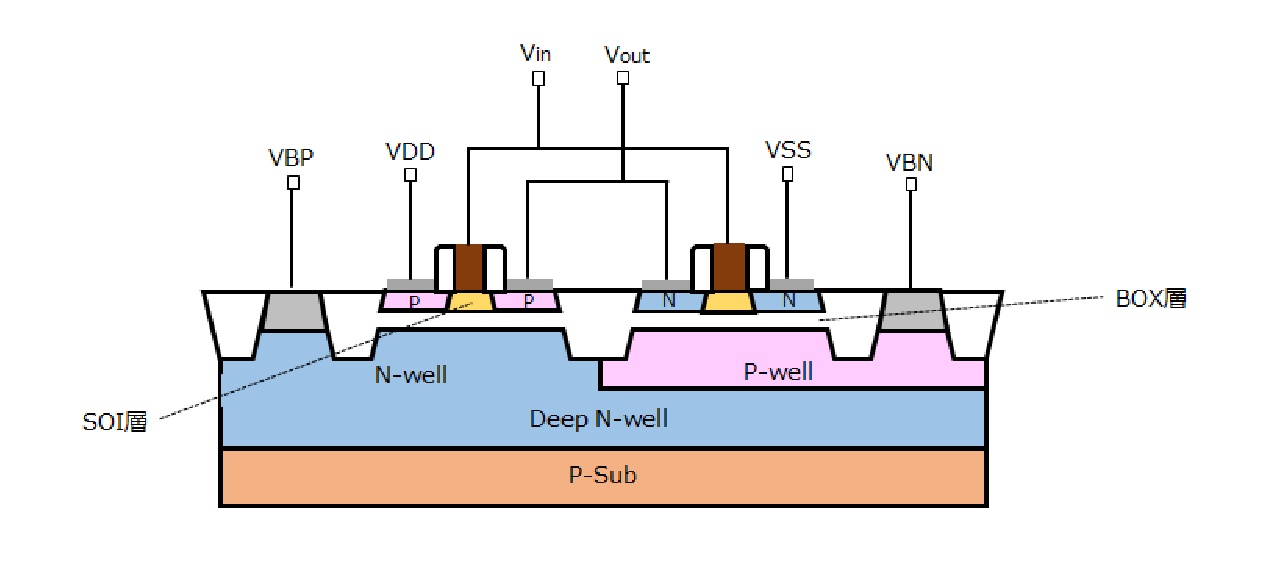
\includegraphics[width=12cm]{./chap2/fig/sotb.eps}
\caption{SOTBトランジスタの構造}
\label{fig:sotb}
\end{figure}
\subsection{ボディバイアス制御}
ボディバイアス電圧のうちnMOS側の電圧を$V_{BN}$、pMOS側の電圧を$V_{PN}$、全体のボディバイアス電圧を$V_{BB}$と呼ぶこととする。nMOS、pMOSのバランスを揃える場合以下の関係が成り立つ。
\begin{eqnarray}
VBN & = & VBB \\
VBP & = & VDD - VBB
\end{eqnarray}

$V_{BB}$の値が負のときをリバースボディバイアス、0のときゼロバイアス、正のときをフォワードボディバイアスと呼び以下のトレードオフがある。
\begin{itemize}
\item リバースボディバイアス
	\begin{itemize}
	\item リーク電流が減少
	\item 遅延時間が増加
	\end{itemize}
\item フォワードボディバイアス
	\begin{itemize}
	\item リーク電流が増加
	\item 遅延時間の減少
	\end{itemize}
\end{itemize}

ボディバイアスの制御とは上記のような性能と電力のバランスを制御することである。
